\chapter{Applications}


\section{BayesCNN for Image Classification}
And now I begin my third chapter here \dots

And now to cite some more people~\citet{Rea85,Ancey1996}

\section{BayesCNN for Image Super Resolution}

The recovery of a \ac{HR} image or video from its \ac{LR} counter part is topic of great interest in digital image processing. This task, referred to as \ac{SR}, finds direct applications in many areas such as HDTV \cite{Goto2014}, medical imaging \cite{Peled2001,shi2013cardiac}, satellite imaging \cite{Thornton2006}, face recognition \cite{Gunturk2003} and surveillance \cite{Zhang2010a}. The global \ac{SR} problem assumes \ac{LR} data to be a low-pass filtered (blurred), downsampled and noisy version of \ac{HR} data. It is a highly ill-posed problem, due to the loss of high-frequency information that occurs during the non-invertible low-pass filtering and subsampling operations. Furthermore, the SR operation is effectively a one-to-many mapping from \ac{LR} to \ac{HR} space which can have multiple solutions, of which determining the correct solution is non-trivial. A key assumption that underlies many \ac{SR} techniques is that much of the high-frequency data is redundant and thus can be accurately reconstructed from low frequency components. \ac{SR} is therefore an inference problem, and thus relies on our model of the statistics of images in question.

Many methods assume multiple images are available as \ac{LR} instances of the same scene with different perspectives, i.e. with unique prior affine transformations. These can be categorised as multi-image \ac{SR} methods \cite{Borman1998a, Farsiu2004} and exploit \emph{explicit redundancy} by constraining the ill-posed problem with additional information and attempting to invert the downsampling process. However, these methods usually require computationally complex image registration and fusion stages, the accuracy of which directly impacts the quality of the result. An alternative family of methods are \ac{SISR} techniques \cite{yang2014single}. These techniques seek to learn \emph{implicit redundancy} that is present in natural data to recover missing \ac{HR} information from a single \ac{LR} instance. This usually arises in the form of local spatial correlations for images and additional temporal correlations in videos. In this case, prior information in the form of reconstruction constraints is needed to restrict the solution space of the reconstruction.

\begin{figure*}[htbp]
\begin{center}
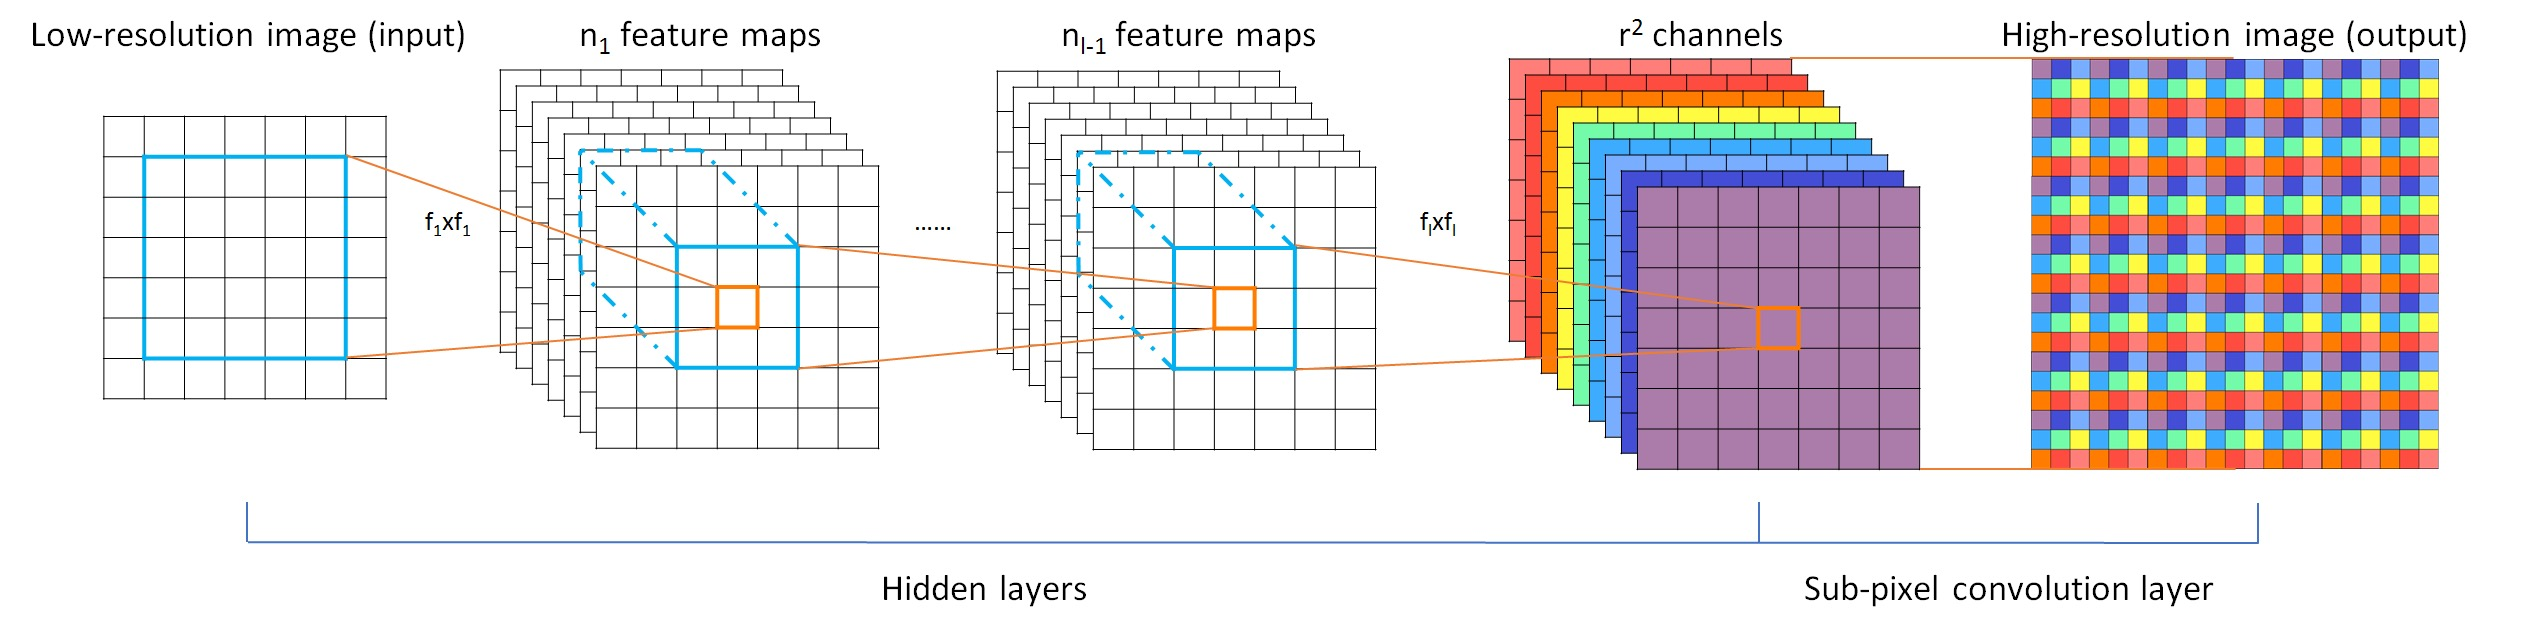
\includegraphics[width=1.0\linewidth]{Chapter6/Figs/networkstructure.jpg}
\caption{The proposed efficient sub-pixel convolutional neural network (ESPCN), with two convolution layers for feature maps extraction, and a sub-pixel convolution layer that aggregates the feature maps from \ac{LR} space and builds the \ac{SR} image in a single step.}
\label{fig:networkstructure}
\end{center}
\end{figure*}

\subsection{Related Work}

The goal of \ac{SISR} methods is to recover a \ac{HR} image from a single \ac{LR} input image \cite{glasner2009super}. Recent popular \ac{SISR} methods can be classified into edge-based \cite{sun2011gradient}, image statistics-based \cite{efrat2013accurate,he2011single,yang2013fast,fernandez2013super} and patch-based \cite{chang2004super,wang2012semi,zhang2012multi,gao2012image,zhu2014single,timofte2014a+,dai2015jointly} methods. A detailed review of more generic \ac{SISR} methods can be found in \cite{yang2014single}. One family of approaches that has recently thrived in tackling the \ac{SISR} problem is sparsity-based techniques. Sparse coding is an effective mechanism that assumes any natural image can be sparsely represented in a transform domain. This transform domain is usually a dictionary of image atoms \cite{Mallat:2008:WTS:1525499,Elad:2010:SRR:1895005}, which can be learnt through a training process that tries to discover the correspondence between \ac{LR} and \ac{HR} patches. This dictionary is able to embed the prior knowledge necessary to constrain the ill-posed problem of super-resolving unseen data. This approach is proposed in the methods of \cite{Yang2010c, Dong2011}. A drawback of sparsity-based techniques is that introducing the sparsity constraint through a nonlinear reconstruction is generally computationally expensive.

Image representations derived via neural networks \cite{krizhevsky2012imagenet,zeiler2014visualizing,simonyan2014very} have recently also shown promise for \ac{SISR}. These methods, employ the back-propagation algorithm \cite{le1990handwritten} to train on large image databases such as ImageNet \cite{russakovsky2014imagenet} in order to learn nonlinear mappings of \ac{LR} and \ac{HR} image patches. Stacked collaborative local auto-encoders are used in \cite{cui2014deep} to  super-resolve the \ac{LR} image layer by layer. Osendorfer et al. \cite{osendorfer2014image} suggested a method for \ac{SISR} based on an extension of the predictive convolutional sparse coding framework \cite{poultney2006efficient}. A multiple layer \ac{CNN} inspired by sparse-coding methods is proposed in \cite{dong2015image}. Chen et. al. \cite{chen2015trainable} proposed to use multi-stage \ac{TNRD} as an alternative to \ac{CNN} where the weights and the nonlinearity is trainable. Wang et. al \cite{wang2015deeply} trained a cascaded sparse coding network from end to end inspired by LISTA (Learning iterative shrinkage and thresholding algorithm) \cite{gregor2010learning} to fully exploit the natural sparsity of images. The network structure is not limited to neural networks, for example, a random forest \cite{schulter2015fast} has also been successfully used for \ac{SISR}.

\section{BayesCNN for Generative Adversarial Networks}

\section{Introduction}

Learning reusable feature representations from large unlabeled datasets has been an area of active research. In the context of computer vision, one can leverage the practically unlimited amount of unlabeled images and videos to learn good intermediate representations, which can then be used on a variety of supervised learning tasks such as image classification. We propose that one way to build good image representations is by training Generative Adversarial Networks (GANs) \citep{Goodfellow2014}, and later reusing parts of the generator and discriminator networks as feature extractors for supervised tasks. GANs provide an attractive alternative to maximum likelihood techniques. One can additionally argue that their learning process and the lack of a heuristic cost function (such as pixel-wise independent mean-square error) are attractive to representation learning. GANs have been known to be unstable to train, often resulting in generators that produce nonsensical outputs. There has been very limited published research in trying to understand and visualize what GANs learn, and the intermediate representations of multi-layer GANs.

In this paper, we make the following contributions
\begin{itemize}  
    \item We propose and evaluate a set of constraints on the architectural topology of Convolutional GANs that make them stable to train in most settings. We name this class of architectures Deep Convolutional GANs (DCGAN)
    \item We use the trained discriminators for image classification tasks, showing competitive performance with other unsupervised algorithms.
    \item We visualize the filters learnt by GANs and empirically show that specific filters have learned to draw specific objects.
    \item We show that the generators have interesting vector arithmetic properties allowing for easy manipulation of many semantic qualities of generated samples.
\end{itemize}

\section{Related Work}
\subsection{Representation Learning from unlabeled data}
Unsupervised representation learning is a fairly well studied problem in general computer vision research, as well as in the context of images. A classic approach to unsupervised representation learning is to do clustering on the data (for example using K-means), and leverage the clusters for improved classification scores. In the context of images, one can do hierarchical clustering of image patches \citep{coates2012learning} to learn powerful image representations. Another popular method is to train auto-encoders (convolutionally, stacked \citep{vincent2010stacked}, separating the what and where components of the code \citep{zhao2015stacked}, ladder structures \citep{rasmus2015semi}) that encode an image into a compact code, and decode the code to reconstruct the image as accurately as possible. These methods have also been shown to learn good feature representations from image pixels. Deep belief networks \citep{lee2009convolutional} have also been shown to work well in learning hierarchical representations.

\subsection{Generating natural images}

Generative image models are well studied and fall into two categories: parametric and non-parametric.

The non-parametric models often do matching from a database of existing images, often matching patches of images, and have been used in texture synthesis \citep{efros1999texture}, super-resolution \citep{freeman2002example} and in-painting \citep{hays2007scene}.

Parametric models for generating images has been explored extensively (for example on MNIST digits or for texture synthesis \citep{portilla2000parametric}). 
However, generating natural images of the real world have had not much success until recently. A variational sampling approach to generating images \citep{kingma2013auto} has had some success, but the samples often suffer from being blurry. Another approach generates images using an iterative forward diffusion process \citep{sohl2015deep}. Generative Adversarial Networks \citep{Goodfellow2014} generated images suffering from being noisy and incomprehensible. A laplacian pyramid extension to this approach \citep{denton2015deep} showed higher quality images, but they still suffered from the objects looking wobbly because of noise introduced in chaining multiple models. A recurrent network approach \citep{gregor2015draw} and a deconvolution network approach \citep{dosovitskiy2014learning} have also recently had some success with generating natural images. However, they have not leveraged the generators for supervised tasks.







    
\fbox{
    \parbox{\textwidth}
    {
        Architecture guidelines for stable Deep Convolutional GANs
        \begin{itemize}
            \item Replace any pooling layers with strided convolutions (discriminator) and fractional-strided convolutions (generator).
            \item Use batchnorm in both the generator and the discriminator.
            \item Remove fully connected hidden layers for deeper architectures.
            \item Use ReLU activation in generator for all layers except for the output, which uses Tanh.
            \item Use LeakyReLU activation in the discriminator for all layers.
        \end{itemize}
    }
}
